\documentclass[fleqn,a4paper,11pt]{article}
\title{\(\chi^2\) and \(t\) probability distributions}
\author{Clive Johnson}

\usepackage[parfill]{parskip}
\usepackage{lmodern}

\usepackage{mathtools}
\usepackage{physics}

\usepackage{tikz}
\usetikzlibrary{quotes,angles}

\DeclareMathOperator{\Normal}{\mathcal N}
\DeclareMathOperator{\prob}{\mathrm P}
\newcommand{\defeq}{\vcentcolon=}
\newcommand*\mean[1]{\overline{#1}}

\begin{document}
\maketitle

Consider a random sample of size \(3\) from a normal distribution:
\begin{equation*}
X_1,X_2,X_3 \sim \Normal(\mu, \sigma^2)
\end{equation*}
and take the sample mean
\begin{equation*}
\mean X \sim \Normal(\mu, \frac{\sigma^2}{3})
\end{equation*}
We can represent this geometrically, as in Figure \ref{fig_1}.

%\pgfsetmacro{\l}{7}
\begin{figure}[h]
\begin{center}
\begin{tikzpicture}
\draw[thick,->] (0,0) -- (7,-1) node[anchor=north west] {\(x_1\)};
\draw[thick,->] (0,0) -- (1,7) node[anchor=south east] {\(x_3\)};
\draw[thick,->] (0, 0) -- (5,4) node[anchor=south west] {\(x_2\)};
\draw[dashed] (0, 0) -- (7,7) node[anchor=south west] {\(x_1 = x_2 = x_3\)};
\coordinate (a) at (4,6);
\coordinate (c) at (5.5,5.5);
\coordinate (b) at (3,3);
\draw[thick] (b) node[anchor=east] {\(C\)}
          -- (a) node[anchor=south east] {\(P\)}
          -- (c) node[anchor=west] {\(M\)};
\draw pic["$\theta$", draw=black, -,
          angle eccentricity=1.5, angle radius=0.8cm]
         {angle=c--b--a};
\draw[densely dashed] (-0.5, 6.5) -- (6.5, 0.5) -- (11.5, 1.5)
                node[anchor=west] {\(x_1 + x_2 + x_3 = 3\mean X\)} --
                      (4.5,7.5) -- cycle;
\end{tikzpicture}
\end{center}
\caption{Geometric representation of sample normal variables}
\label{fig_1}
\end{figure}

So the sample \((X_1, X_2, X_3)\) is point \(P\), the point M is
\((\mean X, \mean X, \mean X)\), the point C is
\((\mu, \mu, \mu)\).

Now \((CM)^2 = 3(\mean X - \mu)^2\) and \\
\((MP)^2 =
  (X_1 - \mean X)^2 + (X_2 - \mean X)^2 + (X_3 - \mean X)^2 =
  2S^2\)

This is because \(S\) is defined as
\(S^2 \defeq \dfrac{\sum_{i=1}^n(X_i - \mean X)}{n - 1}\), where \(n = 3\).

So
\begin{align*}
CM &= (\mean X - \mu)\sqrt 3 \\
MP &= S \sqrt 2
\end{align*}
Note that \(\mean X\) and \(S^2\) occupy mutually perpendicular subspaces
and this corresponds to independence in the probability sense. Note also that
\(S^2\) is drawn from a two dimensional subspace of a 3D normal `swarm'. So it
will actually be the sum of squares of two normally distributed random
variables. So \(2S^2/\sigma^2\) will have a \(\chi^2\) distribution with 2
degrees of freedom.

Now
\begin{equation*}
t = \frac{\mean X - \mu}{\pqty{\frac{S}{\sqrt 3}}}
  = \frac{(\mean X - \mu) \sqrt 3}{S}
  = \frac{CM}{\pqty{\frac{MP}{\sqrt 2}}}
  = \sqrt 2 \cot \theta
\end{equation*}
where \(\theta = \widehat{PCM}\).

\section*{General Results}
Generalising the above in \(n\)-dimensional space:

\(S^2\) and \(\mean X\) are independent random variables.
\begin{align*}
\frac{(n - 1)S^2}{\sigma^2} &\sim \chi_{n - 1}^2 \\
t &= \sqrt{n - 1}\cot \theta
\end{align*}
where \(\theta\) is the angle between the \(n\)-dimensional vectors
\begin{align*}
\overrightarrow{CM} &= (\mean X - \mu,
                        \mean X - \mu,\dotsc,
                        \mean X - \mu) \\
\overrightarrow{CP} &= (X_1 - \mu, X_2 - \mu, \dotsc, X_n - \mu)
\end{align*}
We can then use geometrical methods to derive the pdf for \(t\).

\section*{The pdf for the case \boldmath\(n = 2\)}

\begin{figure}[h]
\begin{center}
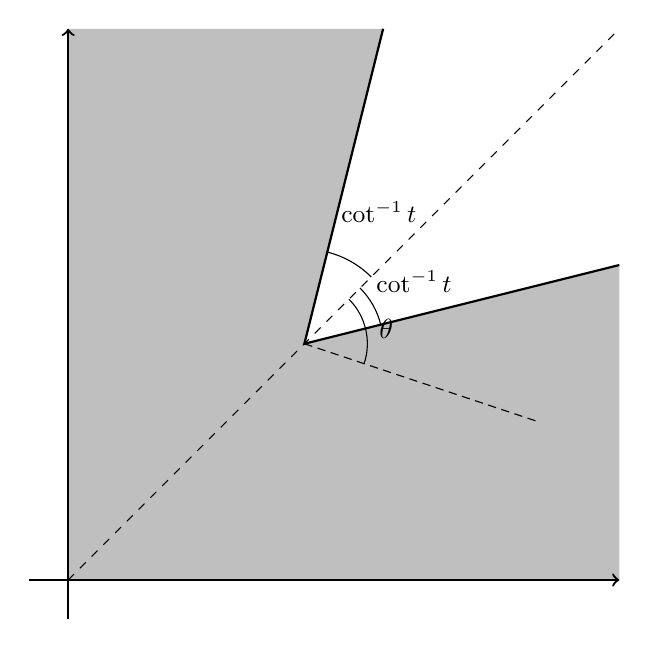
\begin{tikzpicture}
\coordinate (a) at (7, 4);
\coordinate (b) at (3, 3);
\coordinate (c) at (4, 7);
\coordinate (d) at (6, 2);
\coordinate (e) at (7, 7);
\fill[lightgray] (0, 0) -- (7, 0) -- (a) -- (b) -- (c)
              -- (0, 7) -- cycle;
\draw[thick,->] (-0.5,0) -- (7,0);
\draw[thick,->] (0,-0.5) -- (0,7);
\draw[dashed] (0, 0) -- (7, 7);
\draw[thick] (a)--(b)--(c);
\draw pic["\small\(\cot^{-1}t\)", draw=black, -,
          angle eccentricity=1.6, angle radius=1.2cm]
         {angle=e--b--c};
\draw pic["\small\(\cot^{-1}t\)", draw=black, -,
          angle eccentricity=1.6, angle radius=1cm]
         {angle=a--b--e};
\draw[densely dashed] (b)--(d);
\draw pic["\(\theta\)", draw=black, -,
          pic text options={right=0.05cm},
          angle eccentricity=1, angle radius=0.8cm]
         {angle=d--b--e};
\end{tikzpicture}
\end{center}
\caption{Geometry to find the cdf of \(t\)}
\end{figure}

The cdf for \(t\) is given by
\begin{align*}
F(t) &= \prob(\sqrt{2 - 1}\cot \theta < t) \\
     &= \prob(\theta > \cot^{-1} t) \\
     &= \frac{2\pi - 2\cot^{-1} t}{2\pi} \\
     &= 1 - \frac 1\pi \cot^{-1} t
\end{align*}
(using the symmetry of the distributions).

So the pdf for \(t\) with \(2 - 1 = 1\) degrees of freedom is
\begin{equation*}
f(t) = F'(t) = \frac{1}{\pi(1 + t^2)}
\end{equation*}
By much harder geometry, the general pdf for \(t_\nu\) is
\begin{equation*}
f(t) = \frac{C_\nu}{\pqty{1 + \dfrac{t^2}{\nu}}^{(\nu + 1) / 2}}
\end{equation*}
where \(C_\nu\) is a constant such that the area under the curve equals \(1\).

\end{document}
